\documentclass[11pt,a4paper]{report}

\usepackage{listings}
\usepackage{color}
\usepackage{graphicx}

\usepackage{booktabs, multirow} % for borders and merged ranges
\usepackage{soul}% for underlines
\usepackage[table]{xcolor} % for cell colors
\usepackage{changepage,threeparttable} % for wide tables

\usepackage[utf8]{inputenc}          
\usepackage[T1]{fontenc}

\usepackage[english]{babel}
\usepackage{lmodern}                   % optimized print quality
\usepackage{booktabs}                  % for nicer tables
\usepackage{graphicx}                  % to implement jpg images
\usepackage[doublespacing]{setspace}   % for double line brakes
\usepackage{hyperref}
\usepackage{enumitem}
\usepackage{textcomp}
\usepackage{eurosym}
\usepackage{pdflscape}
\usepackage{afterpage}
\usepackage{capt-of}% or use the larger `caption` package


\hypersetup{
    hidelinks
}

\newlength\mystoreparindent
\newenvironment{myparindent}[1]{%
\setlength{\mystoreparindent}{\the\parindent}
\setlength{\parindent}{#1}
}{%
\setlength{\parindent}{\mystoreparindent}
}

\usepackage{geometry}                  % settings for margins
\geometry{left=2.5cm,right=2.5cm,top=2cm,bottom=3cm}

                                       % for literature
\usepackage[authordate,backend=biber,maxcitenames=2]{biblatex-chicago}
\usepackage{graphicx} 
\usepackage{grffile}
\usepackage{csquotes}
\usepackage[normalem]{ulem}


\definecolor{dkgreen}{rgb}{0,0.6,0}
\definecolor{gray}{rgb}{0.5,0.5,0.5}
\definecolor{mauve}{rgb}{0.58,0,0.82}

\lstdefinelanguage{swift}
{
  morekeywords={
    open,catch,@escaping,nil,throws,func,if,then,else,for,in,while,do,switch,case,default,where,break,continue,fallthrough,return,
    typealias,struct,class,enum,protocol,var,func,let,get,set,willSet,didSet,inout,init,deinit,extension,
    subscript,prefix,operator,infix,postfix,precedence,associativity,left,right,none,convenience,dynamic,
    final,lazy,mutating,nonmutating,optional,override,required,static,unowned,safe,weak,internal,
    private,public,is,as,self,unsafe,dynamicType,true,false,nil,Type,Protocol,import,@override,super
  },
  morecomment=[l]{//}, % l is for line comment
  morecomment=[s]{/*}{*/}, % s is for start and end delimiter
  morestring=[b]", % defines that strings are enclosed in double quotes
  breaklines=true,
  escapeinside={\%*}{*)},
  numbers=left,
  captionpos=b,
  breakatwhitespace=true,
  basicstyle=\linespread{1.0}\ttfamily\footnotesize, % https://tex.stackexchange.com/a/102728/129441
}

\lstset{frame=tb,
        language=swift,
        basicstyle=\small\ttfamily,basicstyle=\linespread{0.8}\small\ttfamily,
        aboveskip=20pt,
        belowskip=20pt,
        stepnumber=1,
        showstringspaces=false,
        showspaces=false
        columns=flexible,
        basicstyle={\small\ttfamily},
        numbers=left,
        numberstyle=\tiny\color{gray},
        keywordstyle=\color{blue},
        commentstyle=\color{dkgreen},
        stringstyle=\color{mauve},
        breaklines=true,
        breakatwhitespace=false,
        tabsize=3,
        literate=%
          {€}{\euro}1%
}

\newcommand{\code}{\texttt}


\addbibresource{sources.bib}         % file with sources

%\includeonly{chapters/results}

%\includeonly{chapters/titlepage, chapters/tableofcontents, chapters/introduction, chapters/flutter, chapters/study_design, chapters/implementation, chapters/appendix}
%%%%% END OF SETTINGS %%%%%%%%%%%%%%%%%%%%%%%%%%%%%%%%%%%%%%%%%%%%%%%%%%%%%%%%%%x


\begin{document}

\pagenumbering{roman}                  % small roman page numbers

\thispagestyle{empty}                  % no page number on title page


\begin{center}                         

\textbf{\Huge Flutter and iOS Application Comparison}

\textbf{\large An Empirical Metric Analysis of Performance and User Experience}

\vspace{5cm}

\textbf{\huge Bachelor Thesis}

\vspace{2cm}



\large\centering\doublespacing
\hspace{1.3cm}\begin{tabular}{p{4.2cm}p{0.3cm} p{8.7cm}l}
submitted by: & & Philip Krück\\
Date of Birth: & & 04.11.1998\\
Matriculation Number: & & 3938\\
Company Supervisor: & & Jan Jelschen\\
First Reviewer: & & Dr. Oliver Becker\\
Word Count: & & < 12.000 (text + footnotes) \\
Degree Program: & & B.Sc. Business Informatics (A Track 2018)\\
University: & & Hamburg School of Business Administration\\
Submission Date: & & 09.04.2021\\
Partner Company: & & apploft GmbH\\
\end{tabular}


\vspace{2cm}


\includegraphics[width=7cm]{images/apploft.png} % apploft-Logo

\vspace{0.5cm}


\includegraphics[width=10cm]{images/hsba.png} % HSBA-Logo

\end{center}
%%%%% END OF TITLE PAGE %%%%%%%%%%%%%%%%%%%%%%%%%%%%%%%%%%%%%%%%%%%%%%%%%%%%%%%%%%


%%%%% CHAPTER: ABSTRACT %%%%%%%%%%%%%%%%%%%%%%%%%%%%%%%%%%%%%%%%%%%%%%%%%%%%
\chapter*{Abstract}

To be written... (max: 300 words)

\tableofcontents

%\listoftables

%\listoffigures



\pagenumbering{arabic}

\chapter{Introduction}
\label{section:introduction}
Mobile platforms are dominated by two players - Apple and Google with their respective operating systems iOS and Android. 
Cumulatively, they form a duopoly in the smartphone operating systems market with a combined usage share of 
15.2\% for iOS and 84.8\% for Android in 2020 according to to the International Data Corporation (\cite{IDC2021}).
\\To develop a mobile software application (\textit{app}) for both target platforms, the corresponding development environments and technologies 
are utilized for each platform. This leads to a doubling of cost, development time, and 
the need for knowledge of two different application development paradigms. 
As a result, cross-platform frameworks such as Xamarin (\cite{Xamarin2021}), React Native (\cite{Facebook2021}), and Ionic (\cite{Ionic2021}) have been created. 

%% MOTIVATION FOR CROSS-PLATFORM FRAMEWORKS GENERALLY
The fundamental principle behind these frameworks is the provision of a unified tech stack operating on a single code base leading to increased development speed
while also providing the ability to deploy for both mobile operating systems.

%% PROBLEM WITH CROSS-PLATFORM FRAMEWORKS
Generally, cross-platform frameworks utilize webviews\footnote{Webviews are UI component in both iOS and Android to display web content such as \textit{HTML}, \textit{CSS} and \textit{JavaScript}} or a software bridge to communicate with the underlying host platform plugging into 
native interfaces. In both cases, communication channel delays may occur during app runtime leading to reduced execution speed. In addition, 
cross-platform frameworks deliver abstract interfaces over multiple native interfaces leading to a decreased subset of functionality
and especially impaired UI customizability. These inherent architecture attributes (further see Section \ref{section::other_architectures}) explain
both impeded performance (\cite{Ebone2018} and \cite{Corbalan2019}) and user experience (\cite{Mercado2016} and \cite{Angulo2014}) compared to native technologies.

%% INTRODUCE FLUTTER
However, over the past 2 years one particular cross-platform technology with certain distinct attributes has risen strongly in popularity (\cite{Statista2021}):
Flutter (\cite{FlutterDev20}) is a newly developed open-source UI toolkit by Google. 
It has a nonconventional approach to cross-platform development in that every app ships with the framework's rendering engine (Section ...). 
Thereby, Flutter bypasses host platform communication by avoiding the underlying system app SDK for terms of UI rendering.
Flutter apps are compiled in native binary format which can be directly executed by the mobile computing device (see Section \ref{section::flutter_architecture}).
Furthermore, the framework provides a \textit{"[...] collection of visual, structural, platform, and interactive widgets"} (\textcite{GoogleWidgets2021}) for UI customization.
It seems that Flutter addresses the exact same issues that are generally criticized about cross-platform solutions.

\section{Motivation}
\label{section:motivation}
As a digital agency specialized on native iOS and Android development, \textbf{apploft GmbH} 
(the partnering company of this thesis) (\cite{apploft2021}) is highly interested in Flutter. 
The implications of using this framework could be wide-ranging, including the extension of the services portfolio
to clients with lower budgets.
For example, startups which are unsure about product/market fit (\cite{Andreesen2007}) and held by tight budget constraints are especially keen on reaching 
the maximum number of potential customers with their app. Flutter could be utilized for a fast iteration of a product deployable to 
both mobile platforms. 
Worth noting are the benefits of serving smaller customers like startups which include higher growth potential for long-term cooperation
and risk diversification in apploft's client portfolio.\\
The possible updside of implementing Flutter exceeds the acquisition of small clients. Instead of focusing on platform customization with native tooling, more effort could 
be directed into developing unique custom features.
Furthermore, infrastructure setup, package development and app updates would only be necessary for one codebase.\\
Since the aforementioned economic incentives aren't necessarily company-specific, they are relevant for mobile application developers at large.
Scientifically, this thesis may be the basis for future work on Flutter's architecture attributes and their contribution to runtime performance and UI rendering of frontend toolkits, in general.

\section{Problem Statement}
To the best of the author's knowledge, there are no peer reviewed articles comparing the performance or usability to native apps\footnote{A search for relevant articles has been conducted using Google Scholar, Sci-hub and IEEE Xplore.} since Flutter was first released in March 2018 (\cite{FlutterReleases2020}), 
This leaves an especially interesting gap in the literature, since both aspects are the topmost perceived challenges of cross-platform frameworks considered from an industry-perspective (\cite{BioernHansen2019}).

\section{Thesis Objective} \label{section::thesis_objective}
This thesis will focus on comparing Flutter's framework technology to iOS specifically. The assumption made in this paper, is that mimicking Android-specific appearance and behavior should be rather straightforward as 
both Flutter and Android utilize Google's \textbf{Material design} (\cite{Google2021}) for their default components.
Additionally, testing the framework against iOS is especially interesting as it seems less likely that Flutter would be 
able exploit system specific properties for performance optimization in Apple's closed operating system.\\
The aim of this thesis is derived based on the initially stated problems with cross-platform frameworks and the current lack of research on Flutter's lofty marketing claims to solve those drawbacks.
Specifically, Google's assertion that Flutter can match \textit{"native performance"} and the framework can be utilized for building \textit{"expressive and flexible UI"} (\cite{FlutterDev20})
will both serve as inductively derived hypotheses that shall be empirically verified or falsified individually by this thesis:

\textbf{$H_P$}: The Flutter framework yields comparable \textbf{performance} to native iOS  app development frameworks for iPhone.

\textbf{$H_U$}: Comparable \textbf{user experiences} can be created with Flutter and native iOS frameworks for iPhone.

\section{Methods} \label{section::methods}
An archetypal native mobile app has been chosen as a case study for the evaluation of both hypotheses $H_P$ and $H_U$.
Based on typical mobile application features (explained in detail in Section \ref{section::feature_selection}), \textit{Kickdown} (\cite{Kickdown2021}) - an online car auction app - was chosen for this thesis. 
The app has already been developed for iOS by apploft and released to the App Store in February of 2021 (link to appstore).
For the purposes of comparison, a Flutter equivalent has been developed mimicking the relevant subset of UI and functionality of the original app (see Section \ref{section::feature_selection}). 
Both the original and Flutter replica app are used for subsequent hypothesis testing.


\subsection{Performance comparison}
The assessment of the performance hypothesis $H_P$ has been conducted by profiling specific performance metrics including CPU, GPU and memory usage 
for particular use case flows in the original and Flutter application. 
The profiling results have been analyzed using common statistical techniques.
A further explaination of the measurement process is detailled in Section~\ref{section::performance_comparison_design}.

\subsection{Usability comparison}
The analysis of the usability hypothesis $H_U$ has been evaluated by the means of semi-structured expert interviews.
Specifically, study participants have been be asked to evaluate both the Kickdown iOS and Flutter application clone along various metrics.

A detailed explanation of the interview process is given in Section \ref{section::usability_comparison_design}.

\section{Scope \& Limitations}
The feature set of the implemented app is representative for most, but not every type of app (see Section \ref{section::feature_selection}). 
Therefore the results cannot be generalized to every type of possible app. 
However, they should be seen as indicators of Flutters value as a cross-platform framework for the 
archetypal mobile app. 
Furthermore, the deductively chosen methodology yields the potential of finding adjacent hypothesis which may be
further explored by other researchers.\\
Additionally, the usability study doesn't provide statistical significance due to its qualitative nature. Nevertheless, the depth of detail
in expert interviews is much greater compared to quantitative methods, and unthought of considerations may be suggested by the interviewees.\\
This research attribute is especially compelling given the current research state on the Flutter framework as mentioned above. 

\section{Thesis Structure}
\textit{- TODO: Describe structure of thesis and summarize each chapter. Do this once the other chapters are actually written.}
%In Chapter 2, ...
%Chapter 3 presents


\chapter{Flutter}

\chapter{Methodology and Study Design} \label{chapter::study_design}
This chapter explores the employed methodology for testing both the performance hypothesis $H_P$ and the usability hypothesis $H_U$ (defined in Section \ref{section::thesis_objective}). 
The goal is to explicitly show the reasoning for the chosen methods as well as provide specific method implementation details to aid transparancy about the obtained results discussed in Chapter \ref{chapter::results}.\\
Generally, the employed methodology to achieve the research objective (Section \ref{section::thesis_objective}) is to replicate a relevant subset of functionality of an existing iOS app using Flutter. Thereby, the \textbf{original app} acts as a baseline with which the \textbf{Flutter clone} 
can be comparatively evaluated. Based in this comparison, the research question - whether the Flutter framework can match native performance and provide equivalent usability (Section \ref{section::thesis_objective}) - is answered.
Instead of creating artificial use cases, taking advantage of an existing app provides realistic instances for performance as well as user interface testing.\\
The first section in this chapter (Section \ref{section::facet_selection}) details the decision process for selecting the baseline testing app as well as its feature reduction for further comparison. 
The subsequent two sections (Sections \ref{section::performance_comparison_design} and \ref{section::usability_comparison_design}) explore the specific methods and reasoning for the performance and 
usability comparison respectively.




\section{Baseline App Selection Process} \label{section::facet_selection}
The procedure for choosing the case study app is based on a 4 step filtering process. Each step may be viewed as a constraint
applied upon possible apps progressively reducing the number of potential baseline testing apps:
\begin{enumerate}
    \item The app is built and maintained by apploft. \label{item::constraint_one}
    \item The app includes common application \textbf{facets}. \label{item::constraint_two}
    \item The app uses modern iOS framework technologies. \label{item::constraint_three}
    \item The app conforms to the human interface guidelines (HIG) by Apple (\cite{Apple2021a}). \label{item::constraint_four}
\end{enumerate}
The reasoning behind selecting the above filtering constraints is detailed in the following paragraphs.

\subsection*{Creation and Maintainance by apploft}
This constraint was imposed on the filtering process such that a contact person (apploft
employee) is available for code specific questions.\\
Having a reference to the original source code further provides the ability of implementing the Flutter replica similarly to facilitate comparability with the baseline app.
E.g. a particular algorithm could be implemented similarly in the Flutter application. Thereby, equivalent time and space complexities are produced and 
algorithm implementation can be retracted as a confounding variable.\\
Furthermore, access to the original source code provides the ability to reduce unnecessary features which are irrevalent regarding the hypotheses evaluation. This reduces the complexity of the Flutter replica.

\subsection*{Inclusion of Common Application Features}
The goal of this thesis is to determine whether Flutter is comparable in terms of performance ($H_P$) and usability ($H_U$) for the archetypal mobile app (Section \ref{section::methods}). 
Therefore, only facets commonly appearing in iOS apps are considered for finding the baseline testing app.\\
For the purposes of finding the baseline app, a \textbf{facet} is defined as either
\begin{enumerate}[label=(\alph*)]
    \item a generalizable UI component which is non-trivial, or \label{item::facet_ui}
    \item an underlying technical attribute influencing the user experience. \label{item::technical_attribute}
\end{enumerate}

Trivial UI components \ref{item::facet_ui} such as buttons or text weren't considered \textbf{facets} as they are omnipresent throughout every app.
As for \ref{item::technical_attribute}, a technical attribute has to influence the user experience to be incorporated as the purpose of this thesis is testing Flutter's value as a UI framework (see Section \ref{section::thesis_objective}).
For example, networking can be viewed as a \textbf{facet} if fetched data is displayed via the UI, but is not a \textbf{facet} if the sole purpose of networking within 
an app is to extract analytics data.

\subsection*{Use of Modern iOS Frameworks}
If this constraint were not applied on the filtering process, old iOS technology could be compared to a modernly built Flutter app. 
Therefore, constraining the baseline app to be built with modern iterations of iOS framework technology ensures a reasonable comparison 
against the replica app.\\


\subsection*{Conformance to Human Interface Guidelines}
Conforming to Apple's HIG ensures the original app looks native to the iOS platform.
Since Flutter comes from Google, it probably implements the \textbf{Material Design} (\cite{Google2021}) rather well. Rebuilding an app that conforms to the Apple's design guidelines is the more interesting case.\\
In addition, providing a recognizable UX for iOS users would keep participants in the usability study (detailed in Section \ref{section::usability_comparison_design}) focused on noticing differences instead of 
being distracted by an ambiguous UI.\\
\hfill \break

Based on the above constraints, a small study was conducted looking at 15 apps developed by apploft (constraint \ref{item::constraint_one}) from 9 different iOS App Store categories. 
The factes were extracted into Table \ref{tab::initial_table} by going through each user interface (constraint \ref{item::constraint_two}).
Furthermore, a facet had to appear at least twice before being added as a result.\\
Continuing the filtering process, as per constraint 2 uncommon facets - facets appearing
in less than 50\% of observed apps - are excluded. This reduces the list of facets to the following:

\begin{itemize}
    \item \textbf{Networking} - Interaction with a remote API.
    \item \textbf{Login/Authentication} - User log in meachanism through a UI.
    \item \textbf{Tab navigation} - UI component to quickly switch between different sections of app (\cite{AppleHIGTabBar2021})
    \item \textbf{Hierarchical navigation} - Screens opened on top of previous screens using a Stack structure (\cite{AppleHIGNavigation2021}).
    \item \textbf{Keyboard interaction} - UI for inputing text via a software keyboard.
    \item \textbf{Vertically scrolling collections} - UI collection of items scrolling vertically.
    \item \textbf{Horizontally scrolling collections} - UI collection of items scrolling horizontally.
    \item \textbf{Webview component integration} - Integrated UI component for displaying web content (\cite{AppleHIGWebViews2021}).
\end{itemize}

Out of the 15 initially tested apps, 5 include all of the above \textbf{facets} (conforming to
constraint 1 and 2) (see Table \ref{tab::filtered_table}). Kickdown (see Section ...) is chosen among the remaining 
contestants for the baseline testing app. It was most recently released (Feb 2021) and is therefore built with modern iOS technologies (constraint \ref{item::constraint_three})
and complies to the most recent iteration of the \textbf{Human Interface Guidelines} (constraint \ref{item::constraint_four}).

\subsection{Clone Application Feature Reduction and Implementation} \label{subsection::clone_app_feature_reduction}
The login and signup mechanism - although a common \textbf{facet} - is removed from the original
app for baseline testing. This is due to the fact that textfield and button interaction as well
as networking is already present in other parts of the app and would yield no further insight
regarding the hypotheses evaluation.\\
The Flutter app is implemented as closely as possible to the original application to avoid an
asymmetrical comparison as detailed in Chapter \ref{chapter::implementation}.

\afterpage{
    \clearpage
    \thispagestyle{empty}
    \begin{landscape}
        \begin{center}
            \begin{table}[!htp]
                \caption{Initial Facet Extraction for apploft's Apps}\label{tab::initial_table}
                \tiny
                \begin{tabular}{lrrrrrrrrrrrr}\toprule
                \textbf{} & & &\cellcolor[HTML]{A8A8A8}\textbf{Login/} & &\cellcolor[HTML]{A8A8A8}\textbf{Tab} &\cellcolor[HTML]{A8A8A8}\textbf{Stack} &\cellcolor[HTML]{A8A8A8}\textbf{Keyboard} &\cellcolor[HTML]{A8A8A8}\textbf{Vertically Scrolling} &\cellcolor[HTML]{A8A8A8}\textbf{Horizontally Scrolling} &\textbf{Webview} &\textbf{Camera} \\
                \textbf{App} &\textbf{category} &\cellcolor[HTML]{A8A8A8}\textbf{Networking} &\cellcolor[HTML]{A8A8A8}\textbf{Authentication} &\textbf{Maps} &\cellcolor[HTML]{A8A8A8}\textbf{Navigation} &\cellcolor[HTML]{A8A8A8}\textbf{Navigation} &\cellcolor[HTML]{A8A8A8}\textbf{Interaction} &\cellcolor[HTML]{A8A8A8}\textbf{Collection} &\cellcolor[HTML]{A8A8A8}\textbf{Collection} &\textbf{Components} &\textbf{Interaction} \\\midrule
                bonprix &shopping &1 &1 & &1 &1 &1 &1 &1 &1 & \\
                couponplatz &shopping &1 &1 &1 &1 &1 &1 &1 &1 &1 & \\
                Fernsehlotterie &lifestyle &1 & & &1 &1 &1 &1 &1 &1 & \\
                Gerolsteiner TrinkCheck &health & & &1 & &1 & &1 & &1 & \\
                Hexal Pollenflug &weather &1 & & &1 &1 &1 &1 & &1 & \\
                HIPP Baby &health &1 &1 &1 &1 &1 &1 &1 & &1 &1 \\
                Hipp Bio &food &1 & & & &1 & &1 & &1 &1 \\
                Hipp Buddies app &family & & & & &1 & &1 &1 & & \\
                Hipp Windel &shopping &1 & & &1 &1 & &1 &1 &1 &1 \\
                Kickdown &shopping &1 &1 & &1 &1 &1 &1 &1 &1 & \\
                Lotto Nds. &entertainment &1 &1 & &1 &1 &1 &1 &1 &1 & \\
                Kulturpunkte &travel &1 & &1 & &1 & &1 & & & \\
                Servus TV &entertainment &1 &1 & &1 &1 &1 &1 &1 &1 & \\
                Starcook &food &1 &1 & & &1 &1 &1 &1 &1 &1 \\
                Zeit Online &news &1 &1 & & &1 &1 &1 & &1 & \\
                \midrule
                &9 &\cellcolor[HTML]{A8A8A8}\textbf{13} &\cellcolor[HTML]{A8A8A8}\textbf{8} &\textbf{4} &\cellcolor[HTML]{A8A8A8}\textbf{9} &\cellcolor[HTML]{A8A8A8}\textbf{15} &\cellcolor[HTML]{A8A8A8}\textbf{10} &\cellcolor[HTML]{A8A8A8}\textbf{15} &\cellcolor[HTML]{A8A8A8}\textbf{9} &\cellcolor[HTML]{A8A8A8}\textbf{13} &4 \\
                \bottomrule
                \end{tabular}
            \end{table}
            
            \begin{table}[!htp]
                \caption{Table \ref{tab::initial_table} After Applying Constraint 2}\label{tab::filtered_table}
                \tiny
                \begin{tabular}{lrrrrrrrrrr}\toprule
                \textbf{} & & &\textbf{Login/} &\textbf{Tab} &\textbf{Stack} &\textbf{Vertically Scrolling} &\textbf{Horizontally Scrolling} &\textbf{Webview} & \\
                \textbf{App} &\textbf{category} &\textbf{Networking} &\textbf{Authentication} &\textbf{Navigation} &\textbf{Navigation} &\textbf{Collection} &\textbf{Collection} &\textbf{Components} & \\\midrule
                \cellcolor[HTML]{A8A8A8}\textbf{bonprix} &shopping &1 &1 &1 &1 &1 &1 &1 &\cellcolor[HTML]{A8A8A8}\textbf{7} \\
                \cellcolor[HTML]{A8A8A8}\textbf{couponplatz} &shopping &1 &1 &1 &1 &1 &1 &1 &\cellcolor[HTML]{A8A8A8}\textbf{7} \\
                Fernsehlotterie &lifestyle &1 & &1 &1 &1 &1 &1 &6 \\
                Gerolsteiner TrinkCheck &health & & & &1 &1 & &1 &3 \\
                Hexal Pollenflug &weather &1 & &1 &1 &1 & &1 &5 \\
                HIPP Baby &health &1 &1 &1 &1 &1 & &1 &6 \\
                Hipp Bio &food &1 & & &1 &1 & &1 &4 \\
                Hipp Buddies app &family & & & &1 &1 &1 & &3 \\
                Hipp Windel &shopping &1 & &1 &1 &1 &1 &1 &6 \\
                \cellcolor[HTML]{A8A8A8}\textbf{Kickdown} &shopping &1 &1 &1 &1 &1 &1 &1 &\cellcolor[HTML]{A8A8A8}\textbf{7} \\
                \cellcolor[HTML]{A8A8A8}\textbf{Lotto Nds.} &entertainment &1 &1 &1 &1 &1 &1 &1 &\cellcolor[HTML]{A8A8A8}\textbf{7} \\
                Kulturpunkte &travel &1 & & &1 &1 & & &3 \\
                \cellcolor[HTML]{A8A8A8}\textbf{Servus TV} &entertainment &1 &1 &1 &1 &1 &1 &1 &\cellcolor[HTML]{A8A8A8}\textbf{7} \\
                Starcook &food &1 &1 & &1 &1 &1 &1 &6 \\
                Zeit Online &news &1 &1 & &1 &1 & &1 &5 \\
                \bottomrule
                \end{tabular}
            \end{table}


        \end{center}
    \end{landscape}
}

\subsection{Kickdown App Feature Presentation} \label{section:kickdown_feature_presentation}
\textit{Kickdown} is an online auctioning platform for buying and selling classic and vintag cars (\cite{Kickdown2021}).\\
The original iOS app was built by apploft based on a subset of functionality from the web application and its underlying internal API.
The application is divided into two main sections via tab navigation: the overview and the more screen (see Figure \ref{fig:kickdown_overview_screen} and \ref{fig:kickdown_more_screen}).\\
On the overview, the user has the ability to scroll through all current offerings. Each offering is shown as a card with a hero image 
and some basic information including the title, location, current price and remaining time.\\
Tapping on a posting card brings up a detail view (Figure \ref{fig:kickdown_detail_screen}) for the respective posting.
Besides inspecting detailed information about the particular posting, the user has the option of viewing additional photos in the image gallery (Figure \ref{fig:kickdown_gallery_view}) and placing a bid via a bottom sheet (Figure \ref{fig:kickdown_bid_preparation_screen}).\\
The More screen lets the user login, turn on analytics tracking or open informational webviews such as the data privacy or imprint.





\begin{figure}[htbp]
    \begin{tabular}{p{0.33\textwidth}p{0.33\textwidth}p{0.33\textwidth}}
        \begin{minipage}{.33\textwidth}
            \centering
            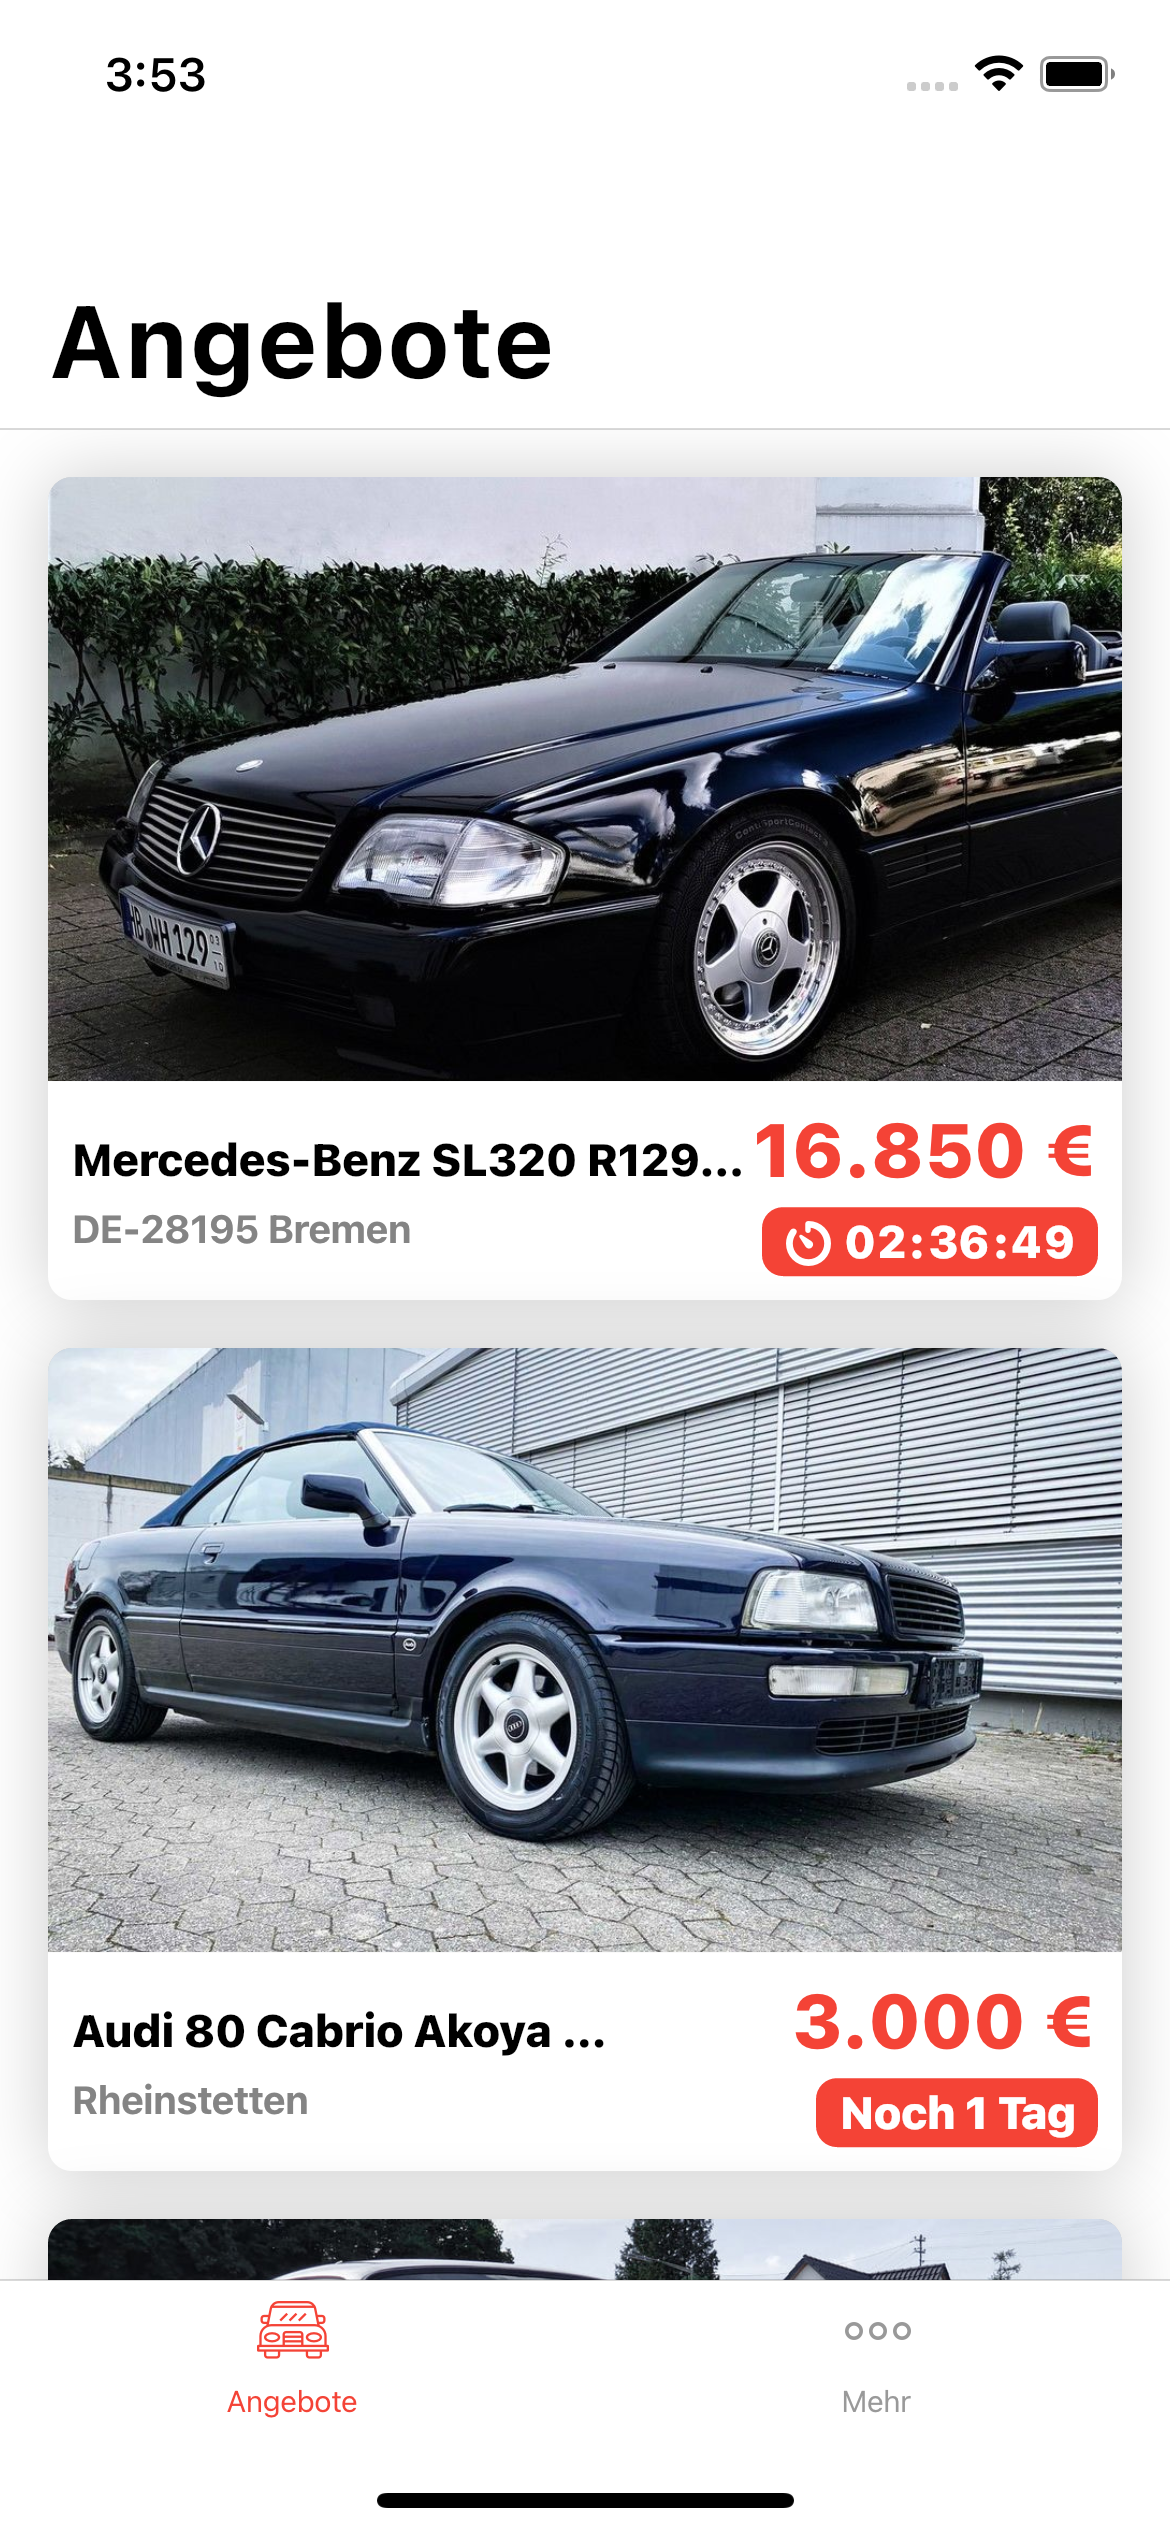
\includegraphics[width=\linewidth, height=300pt]{images/kickdown_presentation/kickdown_overview_screen.png}
            \caption{Kickdown Postings Overview}
            \label{fig:kickdown_overview_screen}
        \end{minipage}
        &
        \begin{minipage}{.33\textwidth}
            \centering
            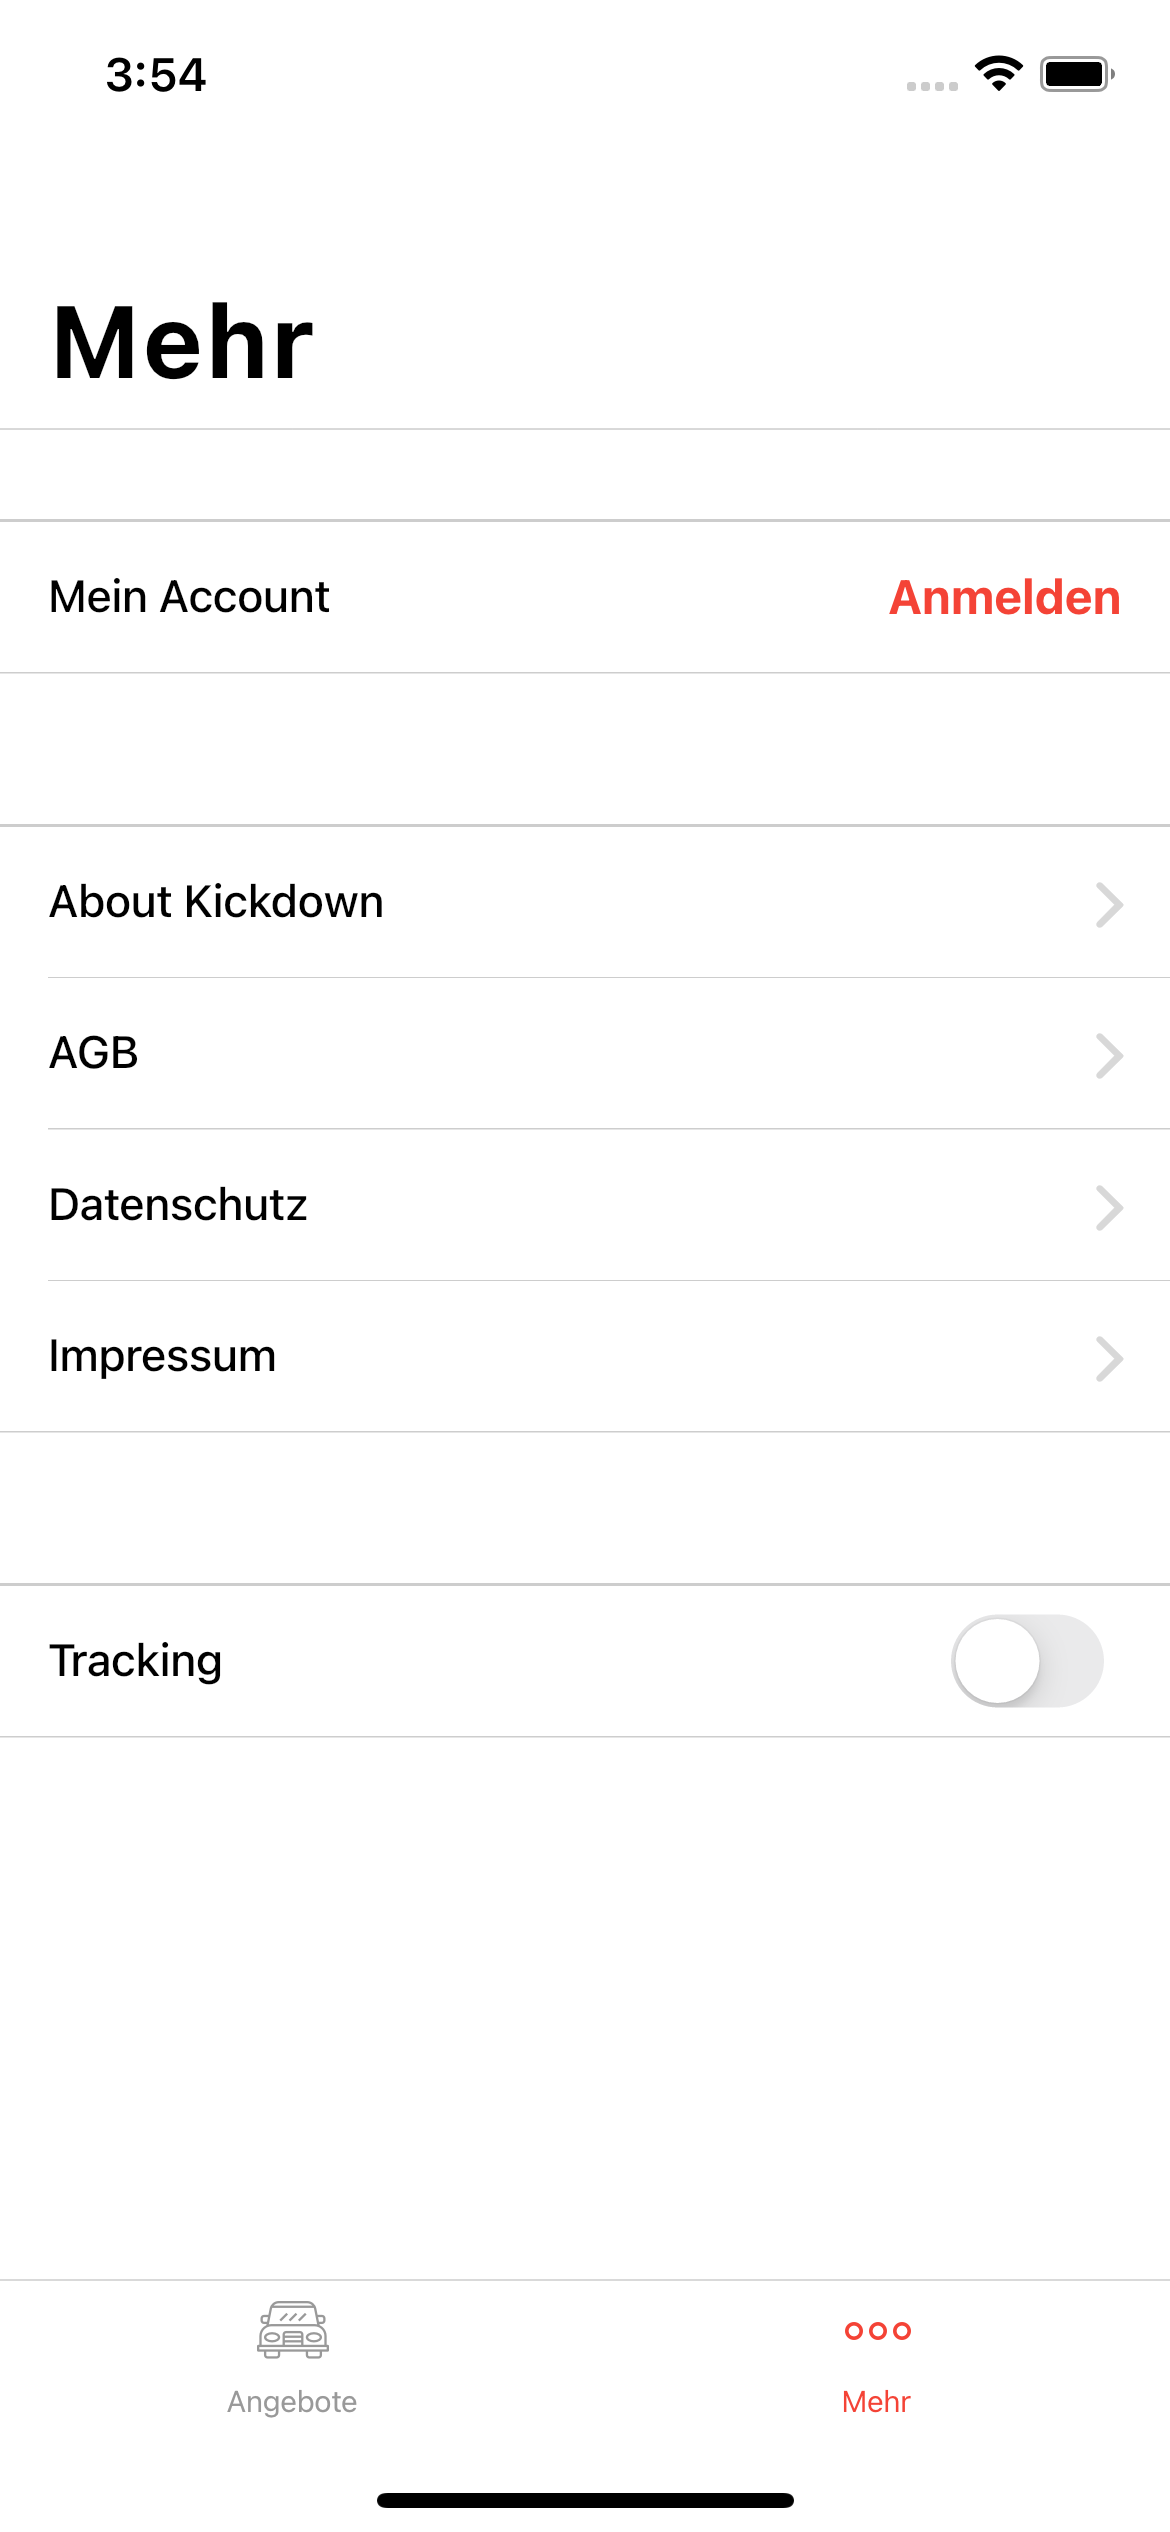
\includegraphics[width=\linewidth, height=300pt]{images/kickdown_presentation/kickdown_more_screen.png}
            \caption{Kickdown More Screen}
            \label{fig:kickdown_more_screen}
        \end{minipage}
        &
        \begin{minipage}{.33\textwidth}
            \centering
            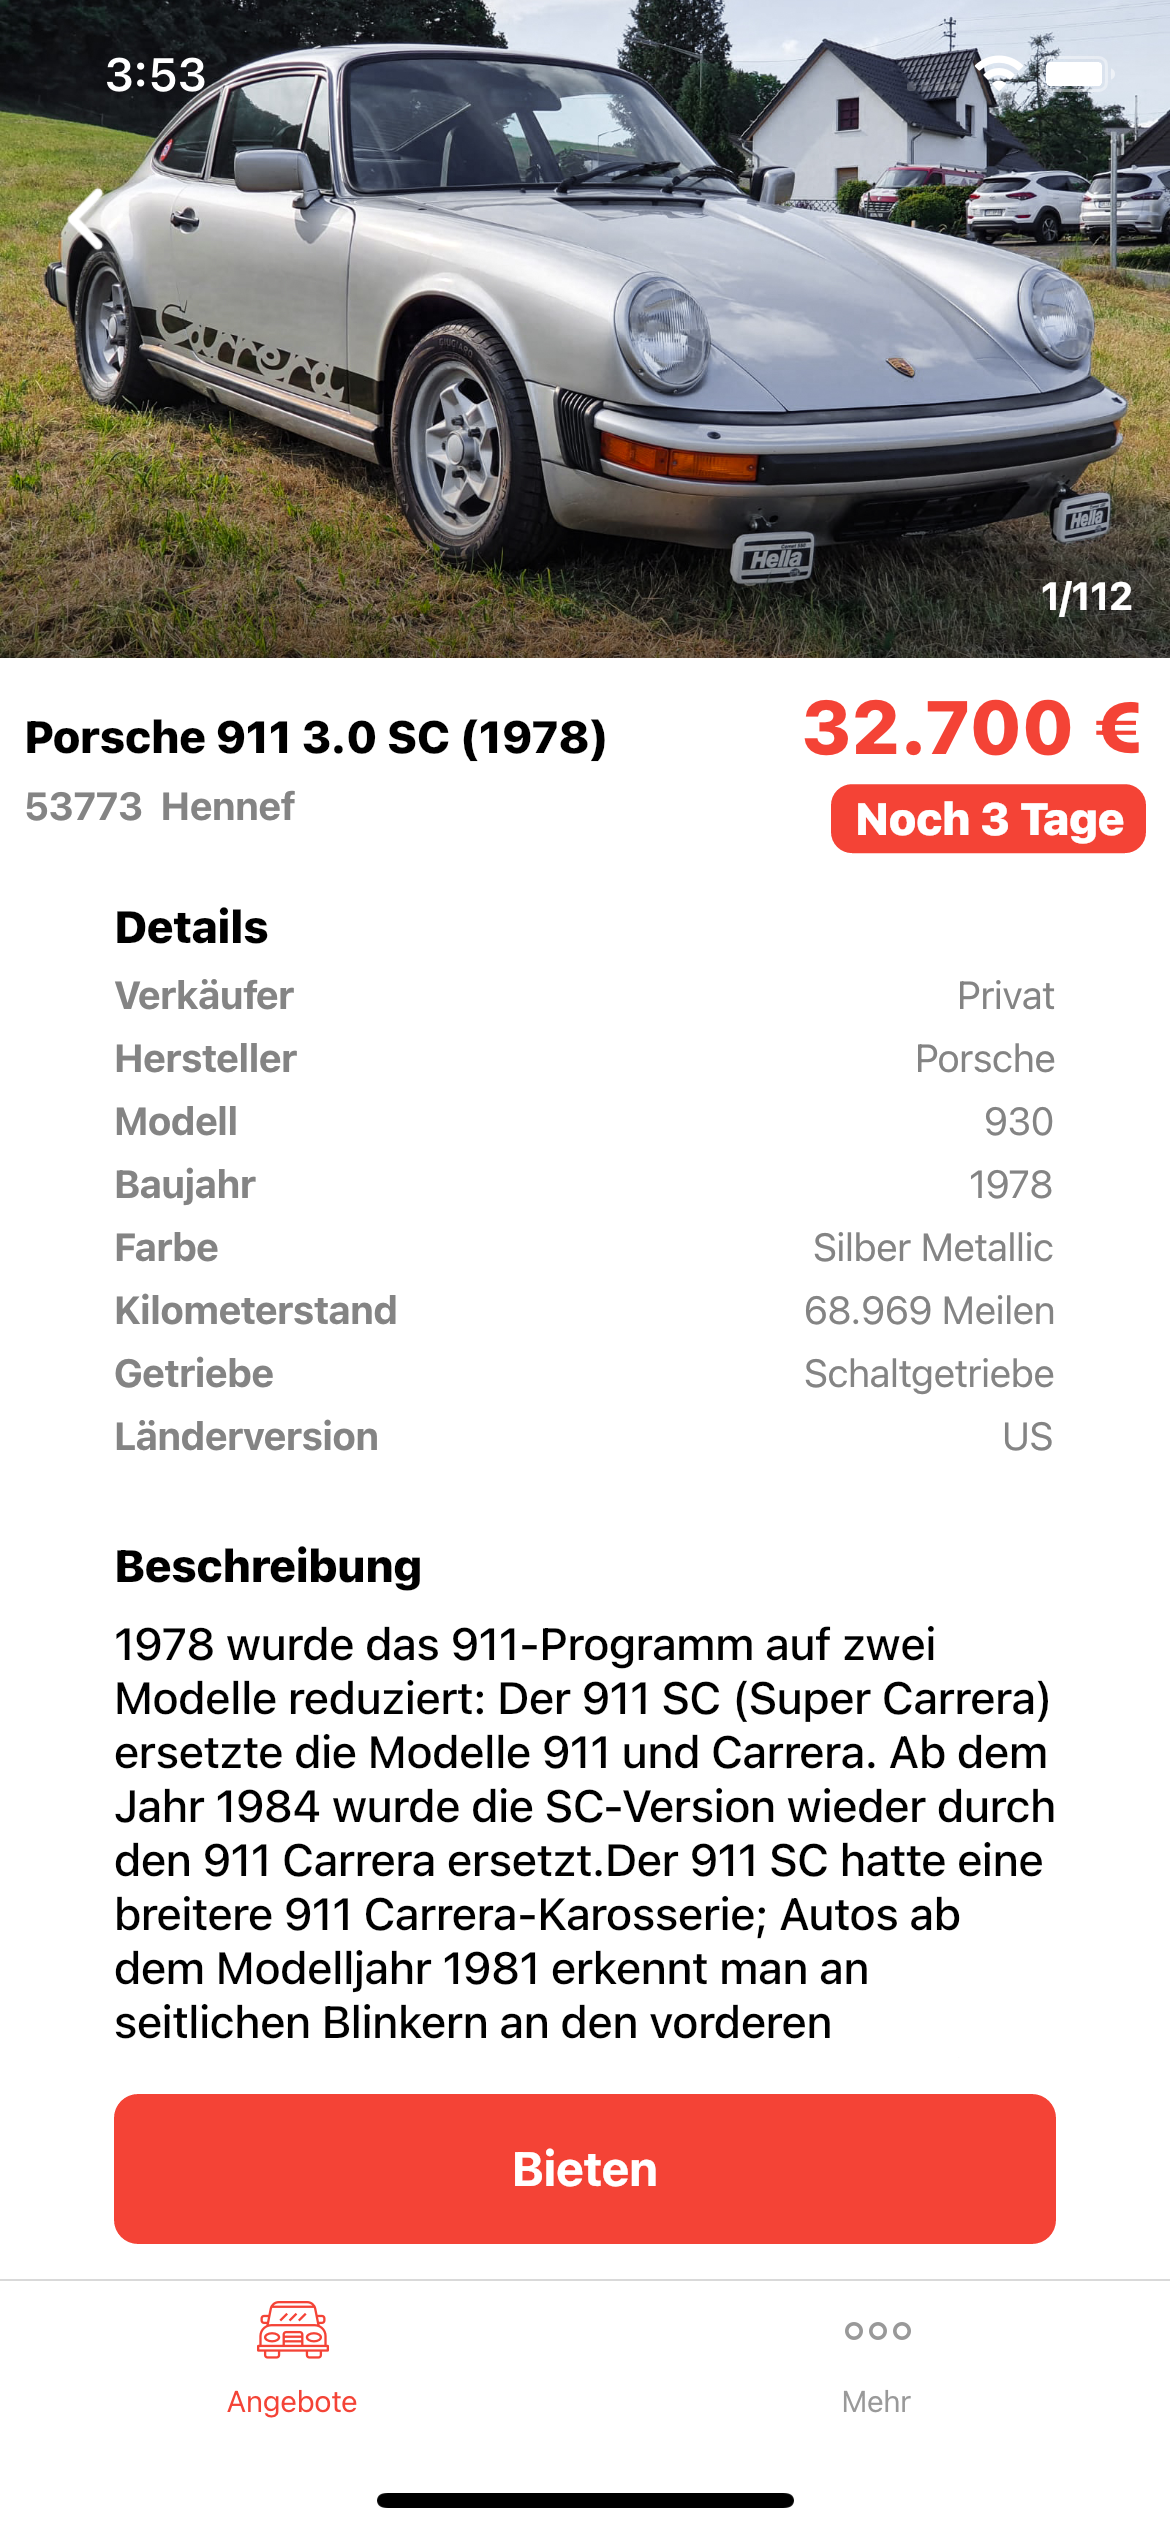
\includegraphics[width=\linewidth, height=300pt]{images/kickdown_presentation/kickdown_detail_screen.png}
            \caption{Kickdown Detail Screen}
            \label{fig:kickdown_detail_screen}
        \end{minipage}
    \end{tabular}
\end{figure}

\begin{figure}[htbp]
    \begin{tabular}{p{0.33\textwidth}p{0.33\textwidth}p{0.33\textwidth}}
        \begin{minipage}{.33\textwidth}
            \centering
            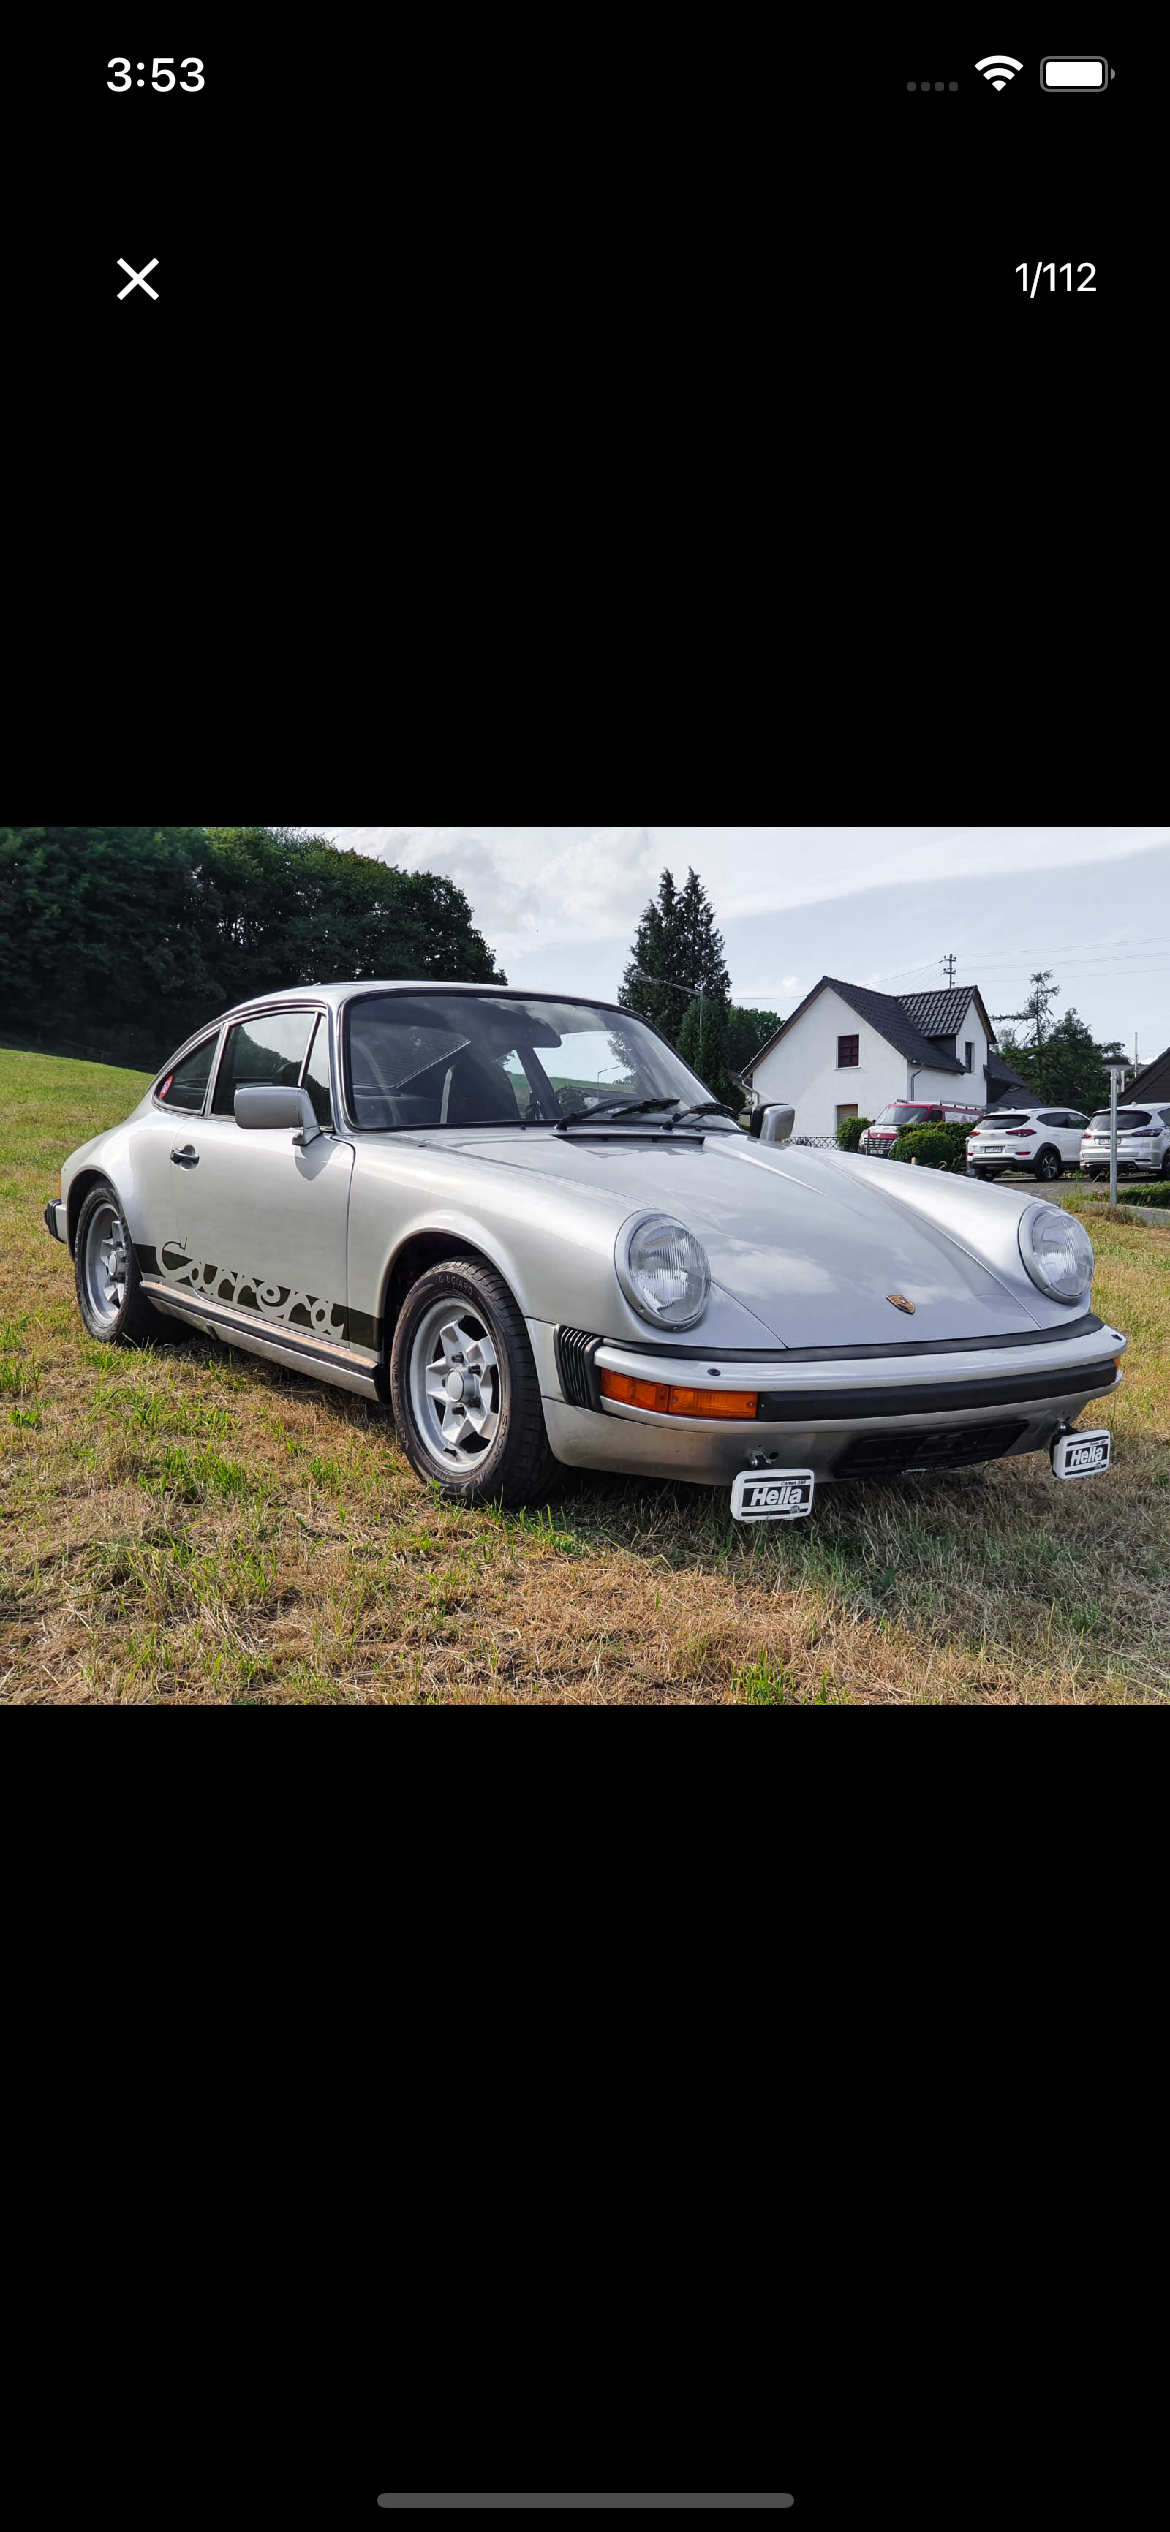
\includegraphics[width=\linewidth, height=300pt]{images/kickdown_presentation/kickdown_gallery.png}
            \caption{Kickdown Gallery View}
            \label{fig:kickdown_gallery_view}
        \end{minipage}
        &
        \begin{minipage}{.33\textwidth}
            \centering
            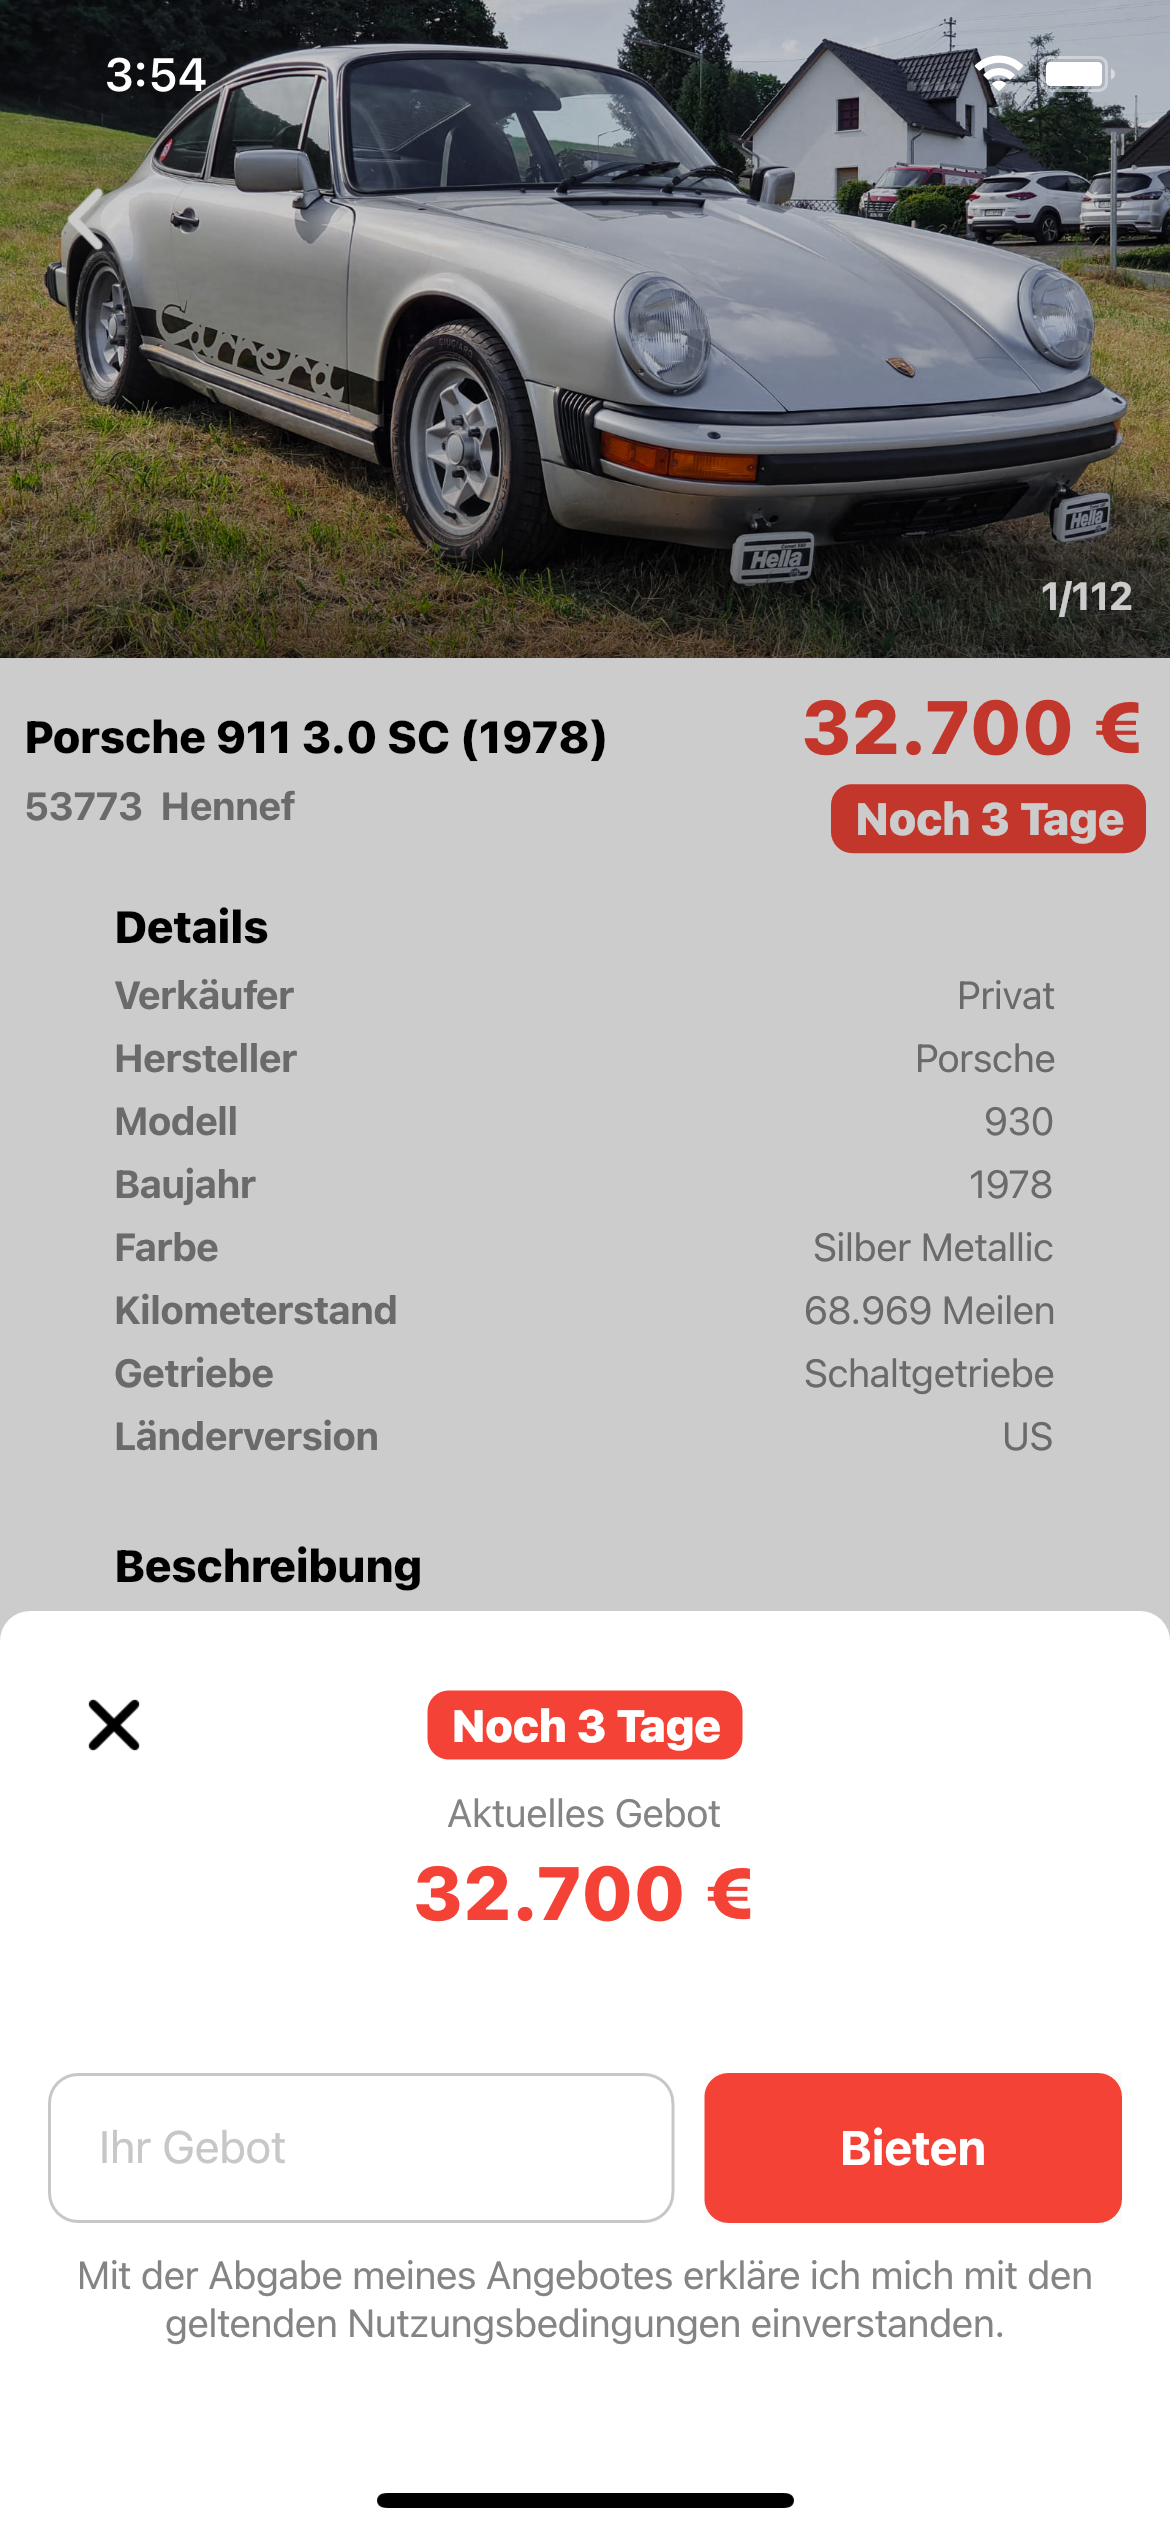
\includegraphics[width=\linewidth, height=300pt]{images/kickdown_presentation/kickdown_bid_preparation_screen.png}
            \caption{Kickdown Bid Preparation Screen}
            \label{fig:kickdown_bid_preparation_screen}
        \end{minipage}
    \end{tabular}
\end{figure}




\section{Performance Comparison} \label{section::performance_comparison_design}
The methodology chosen to empirically test the performance hypthesis $H_P$ (Section \ref{section::thesis_objective}) is a quantitative
measurement of computational resources during app runtime. Measurements are performed for
specific load conditions (i.e use cases). In the process, the original app acts as an empirical
baseline for testing the Flutter replica against.\\
Directly benchmarking system resources provides insight whether the Flutter framework consumes
compute resources efficiently under typically imposed load settings. Furthermore, system
benchmarking metrics are the underlying cause of more ephemeral measures for testing the
system load itself, e.g. page load time. In addition, the chosen compute resources (explained
in Subsection \ref{subsection::selected_measurement_variables}) are easily measured using software tooling (Subsection \ref{subsection::profiling_tooling}) which aids the
objectivity, reliability and validity of this particular study methodology.
Finally, the data is statistically evaluated in order to make inferences about the hypothesis.

\subsection{Selected Performance Measurement Variables} \label{subsection::selected_measurement_variables}
The following paragraphs introduce the selected performance measurement variables. Concretely,
a brief definition is given as well as the reasoning for including the particular metric in
this study with regards to evalutating the performance hypothesis (Section \ref{section::thesis_objective}).

\paragraph*{CPU Utilization}\label{paragraph::cpu_utilization}\hfill \break
CPU utilization is defined as the CPU time (\cite{FSF1988}) of a task
divided by its overall capacity expressed as a percentage. The CPU as well as its integrated GPU\footnote{The GPU is an integrated chip within the System-on-a-Chip (SoC) architecture (\cite{Martin2001}) for all
iPhone processing units (\cite{WikiChip2020}).}
are responsible for graphics rendering related computations. Generally, high CPU usage is an
indicator of insufficient processing power to perform the executed task. Therefore, testing CPU utilization
directly assesses whether Flutter’s framework processing requirements for UI rendering can be
fulfilled given the testing hardware (see Subsection \ref{subsection::measurement_process}).

\paragraph*{Frames per Second}\label{paragraph::fps}\hfill \break
TODO: REWRITE GPU USAGE
Frames per Second (FPS) describes the rate at which the system, and in particular the GPU,
completes rendering individual frames. The FPS rate directly determines the smoothness of UI
animations and transitions (\cite{Google2020}).

\paragraph*{Memory Utilization}\label{paragraph::memory_utilization}\hfill \break
Memory utilization is the percentage of available memory capacity used for a specific task. 
A high level of memory usage negatively impacts performance of running tasks as well as interactive responsiveness (\cite{Ljubuncic2015}).

\subsection{Measurment Process} \label{subsection::measurement_process}
To reduce measurement confounders, the device is restarted before each individual measurement to ensure that all
irrelevant background processes are cancelled.\\
The measurement process for the individual metrics is further split into specific user actions
which are executed and tested on both the iOS and Flutter app separately. These were chosen
to test all relevant facets of the app (see Section \ref{section:kickdown_feature_presentation}) and ensure a sufficient load on the system:
\begin{itemize}
    \item \textbf{app start:} The app is freshly installed on the test device, opened and idle until the visible postings are loaded.
    \item \textbf{scrolling:} On the postings overview screen, the posting cards are vertically scrolled fully to the bottom and subsequently back to the top.
    \item \textbf{detail view:} From the postings overview, the first posting is tapped to navigate to the detail view. Afterwards the back button is tapped to navigate back to the overview.
    \item \textbf{image gallery:} The image gallery of a posting is opened from the detail view of a posting and the first 10 images are viewed by swiping.
\end{itemize}
For each \textbf{user action}, the average of all values over time is recorded. This process is then
repeated 3 times and averaged. The exact number of experiment repetitions was chosen as a
tradeoff between marginal accuracy increase and additional experiment execution time.\\
Furthermore, 2 testing rounds are devised on separate devices. The iPhone 12 Pro and iPhone
6s are chosen as the upper and lower bounds of hardware performance respectively. The lower
bound is defined in this case as per Apples recommendation to set the deployment target to the
current operating system version (iOS 14 at time of writing) minus one (iOS 13) which lists the
iPhone 6s as the oldest supported device (\cite{Apple2021}). iOS 13 is also the minimum deployment target for the Kickdown app.\\

\subsection{Profiling Tools} \label{subsection::profiling_tooling}
\textbf{Xcode Instruments} (\cite{Apple2019}) - a part of the \textbf{Xcode} IDE tool set - are used for profiling the individual metrics. It provides multiple preconfigured
profiling trace instruments.
For the purposes of this thesis, the \textbf{Time Profiler} tool (see Figure \ref{fig:time_profiler_graph} and \ref{fig:time_profiler_table}) is used for CPU (see Paragraph \ref{paragraph::cpu_utilization}),
the \textbf{Allocations} tool (see Figure \ref{fig:allocations_profiler_graph} and \ref{fig:allocations_profiler_table}) for memory usage (see Paragraph \ref{paragraph::memory_utilization}) and \textbf{Core Animation} tool (see Figure \ref{fig:core_animation_profiler_graph} and \ref{fig:core_animation_profiler_table}) for FPS (see Paragraph \ref{paragraph::fps}).
For each profiling tool a graph shows the particular metric quantified over time with an associated table showing the exact numeric values with time stamps.

\begin{figure}[htbp]
    \begin{tabular}{p{0.5\textwidth}p{0.5\textwidth}}
        \begin{minipage}{.5\textwidth}
        \centering
        \includegraphics[width=\linewidth]{images/profiling/time_profiler/time_profiler_graph.eps}
        \caption{Time Profiler Graph}
        \label{fig:time_profiler_graph}
        \end{minipage}
        &
        \begin{minipage}{.5\textwidth}
            \centering
            \includegraphics[width=\linewidth]{images/profiling/time_profiler/time_profiler_table.eps}
            \caption{Time Profiler Table}
            \label{fig:time_profiler_table}
        \end{minipage}
    \end{tabular}
\end{figure}

\begin{figure}[htbp]
    \begin{tabular}{p{0.5\textwidth}p{0.5\textwidth}}
        \begin{minipage}{.5\textwidth}
        \centering
        \includegraphics[width=\linewidth]{images/profiling/allocations_profiler/allocations_graph.eps}
        \caption{Allocations Profiler Graph}
        \label{fig:allocations_profiler_graph}
        \end{minipage}
        &
        \begin{minipage}{.5\textwidth}
            \centering
            \includegraphics[width=\linewidth]{images/profiling/allocations_profiler/allocations_table.eps}
            \caption{Allocations Profiler Table}
            \label{fig:allocations_profiler_table}
        \end{minipage}
    \end{tabular}
\end{figure}

\begin{figure}[htbp]
    \begin{tabular}{p{0.5\textwidth}p{0.5\textwidth}}
        \begin{minipage}{.5\textwidth}
        \centering
        \includegraphics[width=\linewidth]{images/profiling/core_animation/core_animation_graph.eps}
        \caption{Core Animation Profiler Graph}
        \label{fig:core_animation_profiler_graph}
        \end{minipage}
        &
        \begin{minipage}{.5\textwidth}
            \centering
            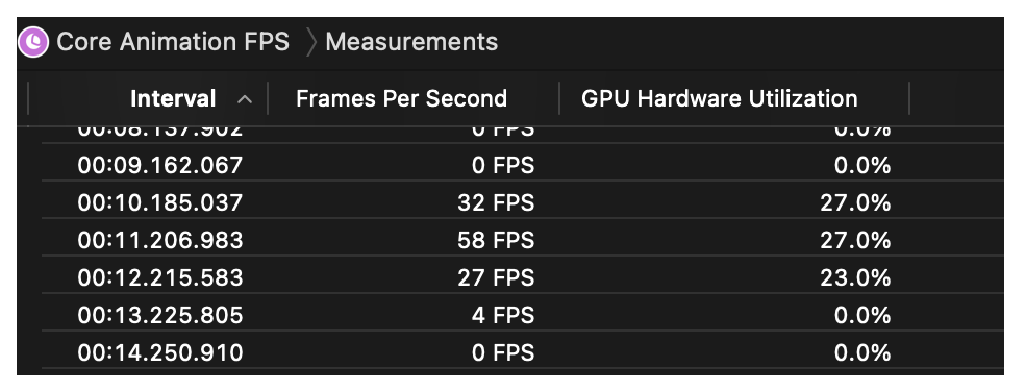
\includegraphics[width=\linewidth]{images/profiling/core_animation/core_animation_table.eps}
            \caption{Core Animation Profiler Table}
            \label{fig:core_animation_profiler_table}
        \end{minipage}
    \end{tabular}
\end{figure}



\subsection{Evaluation Process} \label{subsection::evaluation_process}
To better understand the data gathered, it is subsequently examined using exploratory data
analysis (EDA) (\cite{Tukey1977}). \textit{To be continued a bit...}


\section{User Experience Comparison} \label{section::usability_comparison_design}
%%% Goal %%%
This Section explores the usability hypothesis evaluation methodology. Specifically, laying out
the procedure to answer the question of whether or not the Flutter framework is capable of
reproducing native iOS application user experiences (see Section \ref{section::thesis_objective}).

%%% Problem with measuring UX and why performance results are used %%%
Generally, as UX is built for other humans, any evaluation is prone to subjectivity and perception
biases (\cite{Tversky1974}). Therefore, it is difficult to capture these impressions quantitatively in a reproducable manner.\\
However, the user experience of an app is directly dependant upon sufficiently underlying performance (e.g. for scrolling
fluidity). Therefore the results of the performance comparison (Section \ref{section::performance_comparison}) form the basis of the evaluation of the usability hypothesis $H_U$.
Utilizing a mixed approach as a study methodology combining both the quantitative performance comparison and a qualitative method will draw upon the strengths of both approaches. 

%%% Why I'm using expert interviews %%%
Specifically, \textit{semi structured interviews with subject matter experts} (see \cite{Liebold2009}) are conducted to evaluate the baseline application
with the Flutter replica by asking the participants for differences between the two apps (further explained in Subsection \ref{subsection::interview_guideline}). This methodology has the
advantage of covering predetermined topics relevant to the research question while also allowing spontaneous discussion possibly leading to novel insights.\\
Furthermore, expert interviews are an especially useful approach for scientific explorations
with no or scant preexisting theory (see \cite{Experts2009}).

%%% Number of interviews conducted %%%
As soon as no new perspectives seem to emerge during interviews, no further interviews will be conducted.
This is based on the fact that the method of expert interviews 
aims to provide a breadth of perspectives on a given topic unlike specific quantitative anaylses (see \cite{Liebold2009}).


\subsection{Interview Preliminaries and Technicalities}
The interviews are conducted with employees of apploft. They qualify as subject matter experts in the sense that they have been working in the mobile app industry for multiple years. They come from a variety
of professional backgrounds including UX and UI design, project management as well as software engineering. Furthermore, some interviewees have actually worked on the original app itself. This diversity 
among the study participants is especially relevant in order to explore a breadth of perspectives. 
Due to the ongoing Covid-19 pandemic, the interviews are conducted through video calls, are recoreded with the interviewees consent and the interviewees are asked to share their iPhone screen via Quicktime player (\cite{Apple2014}).
The moderation and recording is facilitated by the author.
For the comparison, the interviewees receive QR codes with which both apps may be downloaded. Behind each distributed code is a downloadable IPA (iOS App Store Package) binary executable file hosted by an HTTP server.
These work exactly the same as any other apps downloaded from the iOS App Store.
Both apps are blindly distributed to the participants as "Kickdown A" and "Kickdown B" in order to remove confirmation bias as a confounder (see \cite{Tversky1974}).

\subsection{Interview Guideline} \label{subsection::interview_guideline}
%% Goal %%%
The interview guideline (see Appendix \ref{section::interview_guideline}) is based on finding out perceptual differences between the iOS baseline and Flutter replica app.

%% Use Cases %%
Just like the performance comparison, use cases associated with particular UI facets form the basis for the evaluation:
\begin{itemize}
    \item \textbf{App Start and Scroll Behavior}
    \item \textbf{Detail Transition, Modal Transition, Textfield interaction}
    \item \textbf{Horizontal Scrolling}
    \item \textbf{Switch Interaction}
\end{itemize}
The interviewees are asked to perform a particular use case for app A and app B. Then they are asked to detail differences between the two apps.
Asking this open-ended question aims at receiving as much information possible about perceptual differences (Cf. \cite[182--185]{Helferrich2011}).
Subsequently, the participant is asked to determine which of the two apps felt more natural (i.e. had a better UX). A determined trivalent response of: "A", "B" or "same" is expected. 
The goal of this question is to get overall impression of the usability. \\
Both questions are asked after each use case execution of the participant. 
To maintain a high participant engagement during interviews, use cases are described in a more captivating way, e.g. "Please find the blue Mercedes SUV in Kickdown A [Wait until participant has found it.]. Now, 
please look for the black BMW convertible in the other app.". 
After each use case, the ordering of app A and B is swapped. E.g. if the first case starts with A, the second starts with B. This choice is made as to avoid recency bias (Cf. \cite{Atkinson1968}).
Furthermore, the ordering is also swapped after each interview. In this way, participant X starts with app A while participant Y starts with B.
Finally, after the last use case, the participant is asked to answer the two questions with regard to the entire application.


\subsection{Interview Evaluation} \label{section::interview_evaluation}
The videos from the interviews are transcribed into a textual format and further processed using \textbf{interview coding}. Thereby, each interview is categorized into semantic themes. These themes among
all interviews are then merged into an overall theme structure - also known as code structure. This code structure forms the basis for the evaluation of the usability hypothesis $H_U$. 
% Todo: Further research this topic.

\chapter{Application Design and Implementation}
- Thesis is not an [Ingenieurswissenschaftliche Arbeit] and thus application design and implementation will be explained from a perspective
a necessary requirement to execute both the performance and UX comparison.
- goal from development perspective was to get implement Flutter as close as possible to the original app in terms of UI\\
- used as many out of the box cupertino widgets as possible for implementation\\
- only deviated from above guideline when absolutely necessary\\
- this was the case when implementing the following features\\
- image gallery (zooming ability), image caching, custom modal iOS 13 presentation)\\s
- Naturally, software implementation complexity may impede performance if unscalable algorithms or memory-inefficient datastructures are chosen.
In order to prevent this bias to be introduced into the experiment, the Flutter app was implemented as closely as possible to the original iOS app. Todo: explain in what way.

- should I explain the general app architecture which was used?(MVVM + Services)\\




\chapter{Results} \label{chapter::results}

\section{Performance Comparison} \label{section::performance_comparison}

\section{Usability Comparison} \label{section::usability_comparison}

\chapter{Summary}
- What are my key findings? What is their significance and implications

\subsection{apploft}
- Byproduct of analysis was the development of a decision guide when choosing
between the development of a native and Flutter mobile app

- Reference back to goal in introduction
- What are the limitations of my research
- Future Research questions
- Outlook


%
%%%%% CHAPTER: INTRODUCTION %%%%%%%%%%%%%%%%%%%%%%%%%%%%%%%%%%%%%%%%%%%%%%%%%%%%
\chapter{Introduction}

%%%%% SECTION: BACKGROUND %%%%%%%%%%%%%%%%%%%%%%%%%%%%%%%%%%%%%%%%%%%%%%%%%%%%
\section{Background}
TODO: give a background on native, cross-platform and Flutters development approach


%%%%% SECTION: BUSINESS CONTEXT %%%%%%%%%%%%%%%%%%%%%%%%%%%%%%%%%%%%%%%%%%%%%%%%%%%%
\section{Business Context}
TODO: give background on apploft and why this thesis is relevant in a business context

%%%%% SECTION: OBJECTIVES AND RESEARCH QUESTIONS %%%%%%%%%%%%%%%%%%%%%%%%%%%%%%%%%%%%%%%%%%%%
\section{Objectives and Research Questions}
RQ 1: Is Flutter a viable alternative for developing a typical medium-sized mobile application?\\
RQ 2: How performant is Flutter in terms of CPU, GPU and memory usage as well as application size compared to a native iOS application?\\
RQ 3: What is the difference of Flutter and iOS development in terms of development complexity?\\



%%%%% SECTION: METHODS %%%%%%%%%%%%%%%%%%%%%%%%%%%%%%%%%%%%%%%%%%%%%%%%%%%%%%%%%%%%%%%%%%
\section{Methods}
\subsection{Theoretical background & Literature Review}
- Theoretical background information and decision considerations are organized through a literature review\\
- Information on subject is collected using online search engines and data bases such as Google Scholar, Sci-hub and IEEE Xplore\\
- Flutter is so new (first stable release in 2018) that it is difficult to find peer-reviewed articles on the subject\\
- Keywords for searching include ...\\
- Information about Fluter specifically was gathered using Gooles official documenation on Flutter and its associated programming language Dart\\
- For further elaboration on specific topics, information is searched through the web and the quality and relevance of is cross examined before use. These include professional blogs and developer community websites.\\

\subsection{RQ1}
- specific prototype development to test proof of concept
\subsection{RQ2}
- The performance analysis is conducted by comparing X tests for each performance metric, on both the Flutter and iOS app\\
- Use mean as measurement of tests for comparison purposes\\
- TODO: Explain which tools etc. were used for comparison (Xcode Tools + Flutter Profiling)\\
\subsection{RQ3}
- Main measurement of code complexity comparison would be Lines of Code in both the iOS and the Flutter app.\\
\textit{- This is quite basic - I will not be able to elaborate too much on this. Maybe this should be part of RQ2?}

%%%%% SECTION: SCOPE + LIMITATION %%%%%%%%%%%%%%%%%%%%%%%%%%%%%%%%%%%%%%%%%%%%%%%%%%%%%%%%
\section{Scope and Limitation}
- RQ1 can actually only be answered for specific app and conclusion cannot be generalized\\
- RQ2 Performance comparison is bound to specific app which includes relevant and typical, but not all general mobile use cases\\
- Therefore, the performance analysis should not be considered to be generalizable to all types of mobile applications\\
- This thesis does not aim to make generalizable claims, but rather evaluate whether Flutter could potentially be a valid alternative for mobile development and if it should be studied further\\

%%%%% SECTION: THESIS STRUCTURE %%%%%%%%%%%%%%%%%%%%%%%%%%%%%%%%%%%%%%%%%%%%%%%%%%%%%%%%
\section{Thesis Structure}
- TODO: Describe structure of thesis and summarize each chapter.


%%%%% CHAPTER: LITERATURE REVIEW %%%%%%%%%%%%%%%%%%%%%%%%%%%%%%%%%%%%%%%%%%%%%%%%%%%%
\chapter{Literature Review}

Was sind die cutting edge findings von anderen researchern? \\
Meinen Beitrag dahingehend erläutern \\
Unbeantwortete Fragen darlegen und Fokus auf die Research Gap meiner Arbeit legen

%%%%% CHAPTER: THEORETICAL BACKGROUND %%%%%%%%%%%%%%%%%%%%%%%%%%%%%%%%%%%%%%%%%%%%%%%%%%%%
\chapter{Theoretical Background}
Why Flutter? How does Flutter work?
- Dartlang -> programming paradigms\\
- Dart VM\\
- JIT and AOT\\
- Cross Compilation\\ 
- Hot Reload\\
- Native performance due to architectural-level performance optimization\\
- Widget tree, Element tree and Render Object tree\\ 
- Rendering Engine + Widget Tree Rendering (Skia)\\
- Widgets\\
- Stateful and Stateless Widgets\\
- Material and Cupertino Design Widgets\\
- State Management + declarative UI\\ 
- setState() + Ephemeral States\\
- Shared App State -> ScopedMode, BLoC, Redux, Provider\\
Background on traditional native iOS app development\\


%%%%% KAPITEL: APPLICATION DESIGN %%%%%%%%%%%%%%%%%%%%%%%%%%%%%%%%%%%%%%%%%%%%%%%%%%%%
\chapter{Application Design}
This thesis does not cover the entire development of the application. It only persents the necessary parts for the purposes of later comparison between the native application.\\
- Requirements (Functional, Non-functional requirements)\\
- UI\\
- Flutter App Architecture\\
- Widget Architecture of Screens\\ 
- Navigation\\
- Utilized package dependencies\\
- API Access and Networking\\
- State Management\\




%%%%% KAPITEL: COMPARATIVE ANALYSIS %%%%%%%%%%%%%%%%%%%%%%%%%%%%%%%%%%%%%%%%%%%%%%%%%%%%
\chapter{Comparative Analysis}
\subsection{Performance Evaluation}
- look at specific actions within app (like scrolling, opening page) for comparison\\
- use "Instruments" from Xcode\\
\subsubsection{CPU usage}
-> Time profiler tool for CPU usage\\
\subsubsection{GPU usage}
-> Core Animation tool for GPU FPS\\
\subsubsection{memory usage}
-> Allocations tool for memory usage\\
\subsubsection{energy usage? basically results from above metrics}
\subsection{Code Complexity}
- LOC\\
- What else?\\





%%%%% KAPITEL: DISCUSSION %%%%%%%%%%%%%%%%%%%%%%%%%%%%%%%%%%%%%%%%%%%%%%%%%%%%
\chapter{Discussion}
Key Findings presentieren und beurteilen in Bezug auf vorige Berücksichtigungen\\
Bedeutung der Findings interpretieren



%%%%% KAPITEL: ZUSAMMENFASSUNG %%%%%%%%%%%%%%%%%%%%%%%%%%%%%%%%%%%%%%%%%%%%%%%%%%%%
\chapter{Summary}
Zusammenfassung der Key Findings sowie deren Signifikanz und Implikationen\\
Kritische Beurteilung möglicher Einschränkungen meiner Forschung\\
Zukünftige Forschungsfragen\\
Outlook\\




%%%%%% KAPITEL: EINIGE HINWEISE %%%%%%%%%%%%%%%%%%%%%%%%%%%%%%%%%%%%%%%%%%%%%%%%%%%%%%
\chapter{Latex Tips und Tricks (To be deleted)}


Dies ist das zweite Kapitel.


\section{Fußnoten}
\label{sec:fussnoten}                 % Label für den Verweis auf diese Section


Erster Abschnitt.\footnote{Wir können eine Fußnote hinzufügen.} 



\section{Verweise auf Kapitel und Abschnitte}


Wir können einen Verweis auf Abschnitt \ref{sec:fussnoten} einfügen.



\section{Tabellen}


Wir können eine Tabelle einfügen, siehe Tabelle \ref{tab:beispieltab}.



\begin{table}[hbt]
\centering
\begin{tabular}{lcr}
\toprule
                 & \multicolumn{2}{c}{Verbundene Zellen} \\
\cmidrule{2-3}
   Erste Spalte  & Zweite Spalte  & Dritte Spalte \\
\midrule
   linksbündig   & zentriert      & rechtsbündig  \\
   ...           & ...            & ...           \\
\bottomrule
\end{tabular}
\caption{Beispiel-Tabelle}
\label{tab:beispieltab}
\end{table}



\section{Abbildungen}


Wir können auch Abbildungen einfügen, siehe Abbildung \ref{fig:beispielabb}.


\begin{figure}[hbt]
\begin{center}

\includegraphics[width=10cm]{images/hsba.png}   % für volle Breite verwendet man [width=\linewidth]
\caption{Beispiel-Abbildung} 
\label{fig:beispielabb}
\end{center}
\end{figure}



\section{Literaturverweise}


Wir können einen Artikel aus einem wissenschaftlichen Journal wie \textcite{Glove89} zitieren, ein Buch ist natürlich auch möglich (\cite{Goldb89}). Wir können auch Verweise auf Seitenzahlen einfügen: \textcite[][p. 78]{Goldb89}.
Außerdem können wir Sammelband-Beiträge wie \textcite{Steen01} und Konferenz-Beiträge wie \textcite{Merkl00} zitieren.
Es ist auch möglich, auf andere Quellen wie etwa Websites zu verweisen
(zum Beispiel \cite{HSBA18}).

Der Chicago-Stil für das Literaturverzeichnis ist in diesem Template bereits voreingestellt, ebenso wie der Auto-Jahr-Zitierstil.
Die Angaben zu den zitierten Quellen müssen in einer separaten Datei gespeichert sein (diese muss die Endung .bib haben).
Diese bib-Datei muss im Dokumentkopf angegeben werden (in diesem Template heißt sie Literatur.bib).


\printbibliography[heading=bibintoc] % print bibliography

%%%%% APPENDIX %%%%%%%%%%%%%%%%%%%%%%%%%%%%%%%%%%%%%%%%%%%%%%%%%%%%%%%
\appendix
\chapter{Appendix}

\section{Interview Guideline}
\subsection{Interview Setup}
\begin{itemize}
    \item brief interviewee about thesis and their role in the research
    \item ask if the interview session may be recorded and further processed for scientific inquiry
    \item ensure technicalities before start of interview with participant:
    \begin{itemize}
        \item the participant's iPhone is sufficiently charged, has been restarted and is in "Do Not Disturb" mode
        \item the participant has installed Quicktime player on their iPhone and are sharing it with their MacBook
        \item the participant is sharing their MacBook screen in the video call
        \item the participant has received the QR codes for kickdown A and B
    \end{itemize}
    \item ask the participant if the recording may started
\end{itemize}

\subsection{Background Questions}
Ask the participant about their...
\begin{itemize}
    \item job role
    \item years of experience in the mobile app industry
    \item previous experience with the Kickdown application
\end{itemize}

\subsection{Main Interview}
\paragraph*{App Start and Scroll Behavior}\hfill \break
\textbf{Instructions}
\begin{itemize}
    \item Please open Kickdown (A/B) and find the [color] [brand] [attribute] car.
    \item Please open Kickdown (A/B) and find the [color] [brand] [attribute] car.
\end{itemize}

\textbf{Questions}
\begin{enumerate}
    \item Are there any differences in terms of user experience in any way between the two apps?
    \item If you had to pick one experience over the other, which would you choose (A or B)?
\end{enumerate}

\paragraph*{Detail Transition, Modal Transition, Textfield interaction}\hfill \break
\textbf{Instructions}
\begin{itemize}
    \item Please stay in Kickdown (A/B) and tap on a car of your choice. Bid on the car with an amount of your choice.
    \item Please repeat the process for the Kickdown (A/B). You may choose another car and enter a different amount.
\end{itemize}

\textbf{Questions}
\begin{enumerate}
    \item Are there any differences in terms of user experience in any way between the two apps?
    \item If you had to pick one experience over the other, which would you choose (A or B)?
\end{enumerate}


\paragraph*{Horizontal Scrolling}\hfill \break
\textbf{Instructions}
\begin{itemize}
    \item Please stay in Kickdown (A/B) and open the first posting. Find the picture with the [insert item].
    \item Please open Kickdown (A/B) and open the second posting. Find the picture with the [insert item].
\end{itemize}

\textbf{Questions}
\begin{enumerate}
    \item Are there any differences in terms of user experience in any way between the two apps?
    \item If you had to pick one experience over the other, which would you choose (A or B)?
\end{enumerate}

\paragraph*{    }\hfill \break
\textbf{Instructions}
\begin{itemize}
    \item Please stay in Kickdown (A/B) and use the tab navigation to navigate to the "More Screen". Please turn Tracking on.
    \item Please repeat the process for Kickdown (A/B)
\end{itemize}

\textbf{Questions}
\begin{enumerate}
    \item Are there any differences in terms of user experience in any way between the two apps?
    \item If you had to pick one experience over the other, which would you choose (A or B)?
\end{enumerate}


\paragraph*{Overall}\hfill \break
\textbf{Instructions}
\begin{itemize}
    \item You may test out any functionality of the app that you would like to have.
    \item \textit{The following questions regard their impression of the entire app}
\end{itemize}

\textbf{Questions}
\begin{enumerate}
    \item Are there any differences in terms of user experience in any way between the two apps?
    \item If you had to pick one experience over the other, which would you choose (A or B)?
\end{enumerate}

%\begin{center}
    \chapter*{Ehrenwörtliche Erklärung}
    \begin{flushleft}

    
    I hereby declare that I\\
    1. wrote this bachelor's thesis without the assistance of others; \\
    2. have marked direct quotes used from the literature and the use of ideas of other authors at the corresponding locations in the thesis;\\
    3. have not presented this thesis for any other exam.\\
    
    I acknowledge that a false declaration will have legal consequences.\\[1cm]
    
    
\includegraphics[width=5cm]{images/signature.jpeg}\\
    Hamburg, 09.04.2021 \\[1cm]
    
    I accept that HSBA may check the originality of my work using a range of manual and computer based techniques, including transferring and storing my submission in a database for the purpose of data-matching to help detect plagiarism.
    \\[1cm]
    
    
\includegraphics[width=5cm]{images/signature.jpeg}\\
    Hamburg, 09.04.2021
    \end{flushleft}
    
    
\end{center}

\end{document}

